% Pre-ambulo
\documentclass[a4paper, 12pt]{abnt}

\usepackage[brazil]{babel}
\usepackage[utf8]{inputenc}
\usepackage[T1]{fontenc}
\usepackage{dsfont}
\usepackage{amssymb,amsmath}
\usepackage{multirow}
\usepackage[alf]{abntcite}
\usepackage[pdftex]{color, graphicx}
\usepackage{colortbl}
\usepackage{url}
\usepackage{abnt-alf}
\usepackage{abntcite}
\usepackage{algorithm}
\usepackage{algorithmic}
%\usepackage{alg}
%\usepackage{hyperref}


% Redefinicao de instrucoes
\floatname{algorithm}{Algoritmo}
\renewcommand{\algorithmicrequire}{\textbf{Entrada:}}
\renewcommand{\algorithmicensure}{\textbf{Saída:}}
\renewcommand{\algorithmicend}{\textbf{fim}}
\renewcommand{\algorithmicif}{\textbf{se}}
\renewcommand{\algorithmicthen}{\textbf{então}}
\renewcommand{\algorithmicelse}{\textbf{senão}}
\renewcommand{\algorithmicfor}{\textbf{para}}
\renewcommand{\algorithmicforall}{\textbf{para todo}}
\renewcommand{\algorithmicdo}{\textbf{faça}}
\renewcommand{\algorithmicwhile}{\textbf{enquanto}}
\renewcommand{\algorithmicloop}{\textbf{loop}}
\renewcommand{\algorithmicrepeat}{\textbf{repetir}}
\renewcommand{\algorithmicuntil}{\textbf{até que}}
\renewcommand{\algorithmiccomment}[1]{\% #1}


% Definicao da lista de simbolos
% \simb[entrada na lista de simbolos]{simbolo}:
% Escreve o simbolo no texto e uma entrada na lista de simbolos.
% Se o parametro opcional e omitido, usa-se o parametro obrigatorio.
\newcommand{\simb}[2][]
{%
	\ifthenelse{\equal{#1}{}}
	{\addcontentsline{los}{simbolo}{#2}}
	{\addcontentsline{los}{simbolo}{#1}}#2
}
% Para aceitar comandos com @ (at) no nome
\makeatletter 
% \listadesimbolos: comando que imprime a lista de simbolos
\newcommand{\listadesimbolos}
{
	\pretextualchapter{Lista de símbolos}
	{\setlength{\parindent}{0cm}
	\@starttoc{los}}
}
% Como a entrada sera impressa
\newcommand\l@simbolo[2]{\par #1}
\makeatother


% Definicao da lista de abreviaturas e siglas
% \abrv[entrada na lista de simbolos]{abreviatura}:
% Escreve a sigla/abreviatura no texto e uma entrada na lista de abreviaturas e siglas.
% Se o parametro opcional e omitido, usa-se o parametro obrigatorio.
\newcommand{\abrv}[2][]
{%
	\ifthenelse{\equal{#1}{}}
	{\addcontentsline{loab}{abreviatura}{#2}}
	{\addcontentsline{loab}{abreviatura}{#1}}#2
}
% Para aceitar comandos com @ (at) no nome
\makeatletter 
% \listadeabreviaturas: comando que imprime a lista de abreviaturas e siglas
\newcommand{\listadeabreviaturas}
{
	\pretextualchapter{Lista de abreviaturas e siglas}
	{\setlength{\parindent}{0cm}
	\@starttoc{loab}}
}
% Como a entrada sera impressa
\newcommand\l@abreviatura[2]{\par #1}
\makeatother


% \listofalgorithms: comando que imprime a lista de algoritmos
\renewcommand{\listalgorithmname}{Lista de algoritmos}


% Hifenização de palavras feita de forma incorreta pelo LaTeX
\hyphenation{PYTHON ou-tros}


% Inicio do documento
\begin{document}

	\frenchspacing
	
	% Capa (arquivo Includes/Capa.tex)
	% Capa
% Proteção externa do trabalho e sobre a qual se imprimem as informações indispensáveis 
% à sua identificação.

% Especificação da capa
\begin{titlepage}
	\begin{center}
		
		% Cabeçalho (não deve ser modificado)
		% Contém o brasão da Universidade, o logotipo do Departamento, além dos dados
		% relacionados à vinculação do aluno (Universidade, Centro, Departamento e Curso)
		\begin{minipage}{2.3cm}
			\begin{center}
				
\includegraphics[width=2.25cm, height=2.68cm]{Imagens/Brasao-UFRN.jpg}
			\end{center}
		\end{minipage}
		\begin{minipage}{11.15cm}
			\begin{center}
				\begin{espacosimples}
					{\small \ \\
                       \textsc{Universidade Federal do Rio Grande do Norte}		   			\\
							  \textsc{Centro de Ciências Exatas e da Terra}					\\
							  \textsc{Departmento de Informática e Matemática Aplicada}	   	\\
							  \textsc{Disciplina de Linguagens Formais e Autômatos}}   				\\
				\end{espacosimples}
			\end{center}
		\end{minipage}
		\begin{minipage}{2.3cm}
			\begin{center}
				
\includegraphics[width=2.52cm, height=1.96cm]{Imagens/Logotipo-DIMAp.png}
			\end{center}
		\end{minipage}
			
		\vspace{6cm}
						
		% Título do trabalho
		{\setlength{\baselineskip}%
		{1.3\baselineskip}
		{\LARGE \textbf{Análise do uso de RegEx na biblioteca Glycowork}}\par}
			
		\vspace{3cm}
			
		% Nome do aluno (autor)
		{\large \textbf{Andriel Vinicius de Medeiros Fernandes, Gabrielle de Vasconcelos Borja, Jeremias Pinheiro de Araújo Andrade, Lucas Vinicius Dantas de Medeiros, Maria Paz Marcato, Ramon Cândido Jales de Barros}}
						
		\vspace{6cm}
		
		% Local da instituição onde o trabalho deve ser apresentado e ano de entrega do mesmo
		Natal-RN\\Outubro, 2025 
	\end{center}
\end{titlepage}

	% Folha de rosto (arquivo Includes/FolhaRosto.tex)
	% Folha de rosto
% Contém os elementos essenciais à identificação do trabalho.

% Título, nome do aluno e respectivo orientador e filiação
\titulo{\Large{Análise do Glycan RegEx e o uso de expressões regulares na biblioteca Glycowork}}
\autor{Andriel Vinicius de Medeiros Fernandes, \\
   Gabrielle de Vasconcelos Borja, \\
   Jeremias Pinheiro de Araújo Andrade, \\
   Lucas Vinicius Dantas de Medeiros, \\
   María Paz Marcato, \\
   Ramon Cândido Jales de Barros \\}
\instituicao
{
   DIMAp -- Departamento de Informática e Matemática Aplicada\par
   CCET -- Centro de Ciências Exatas e da Terra\par
   UFRN -- Universidade Federal do Rio Grande do Norte }

% Natureza do trabalho (não deve ser modificada)
\comentario
{
   Pesquisa elaborada e apresentada para a disciplina DIM0606 - Linguagens Formais e Autômatos, ofertada pelo Departamento de Informática e Matemática Aplicada da Universidade Federal do Rio Grande do Norte e ministrada no semestre 2025.2 pelo Prof. Dr. Valdigleis da Silva Costa, como requisito parcial para a obtenção de nota para a 1ª unidade.   %Tese de Doutorado apresentada ao Programa de Pós-Graduação em Sistemas e Computação do Departamento de Informática e Matemática Aplicada da Universidade Federal do Rio Grande do Norte como requisito parcial para a obtenção do grau de Mestre em Sistemas e Computação.\bigskip\\
}

% Local e data
\local{Natal-RN}
\data{Outubro, 2025}

\folhaderosto	
	
	% Resumo em língua vernacula (arquivo Includes/Resumo.tex)
	% TODO: remover ou realmente usar?
	% Resumo em língua vernácula
\begin{center}
	{\Large{\textbf{Análise do uso de RegEx na biblioteca Glycowork}}}
\end{center}

\vspace{1cm}

\begin{flushright}
	Autores: Andriel Vinicius de Medeiros Fernandes, \\
		Gabrielle de Vasconcelos Borja, \\
		Jeremias Pinheiro de Araújo Andrade, \\
		Lucas Vinicius Dantas de Medeiros, \\
		María Paz Marcato, \\
		Ramon Cândido Jales de Barros \\
	Professor: Valdigleis
\end{flushright}

\vspace{1cm}

\begin{center}
	\Large{\textsc{\textbf{Resumo}}}
\end{center}

\noindent O resumo deve apresentar de forma concisa os pontos relevantes de um texto, fornecendo uma visão rápida e clara do conteúdo e das conclusões do trabalho. O texto, redigido na forma impessoal do verbo, é constituído de uma seqüência de frases concisas e objetivas e não de uma simples enumeração de tópicos, não ultrapassando 500 palavras, seguido, logo abaixo, das palavras representativas do conteúdo do trabalho, isto é, palavras-chave e/ou descritores. Por fim, deve-se evitar, na redação do resumo, o uso de parágrafos (em geral resumos são escritos em parágrafo único), bem como de fórmulas, equações, diagramas e símbolos, optando-se, quando necessário, pela transcrição na forma extensa, além de não incluir citações bibliográficas.

\noindent\textit{Palavras-chave}: Palavra-chave 1, Palavra-chave 2, Palavra-chave 3. 
	
	% Lista de figuras
	\listoffigures

	% Lista de tabelas
	\listoftables
	
	% Lista de abreviaturas e siglas
	\listadeabreviaturas
	
	% Lista de algoritmos (se houver)
	% Devem ser incluídos os pacotes algorithm e algorithmic
	% \listofalgorithms
	
	% Sumário
	\sumario

	% Parte central do trabalho, englobando os capítulos que constituem o mesmo
	% Os referidos capítulos devem ser organizados dentro do diretório "Capítulos"

	% Capitulo 1: Introdução (arquivo Includes/Introducao.tex)
	% Introdução
\chapter{Introdução}

A introdução é a parte inicial do texto e que possibilita uma visão geral de todo o trabalho, devendo constar a delimitação do assunto tratado, objetivos da pesquisa, motivação para o desenvolvimento da mesma e outros elementos necessários para situar o tema do trabalho.

\section{Organização do trabalho}

Nesta seção deve ser apresentado como está organizado o trabalho, sendo descrito, portanto, do que trata cada capítulo.
	
	% Capitulo 2: Segundo capítulo (arquivo Includes/Capitulo2.tex)
	% Capítulo 2
\chapter{Capítulo 2}

Neste capítulo, descrevemos o funcionamento do sistema \texttt{Glycan RegEx}
implementado no módulo \texttt{glycowork.motif.regex}, suas funções principais,
o papel das expressões regulares e as vantagens do uso desse sistema.

O \texttt{Glycan RegEx}, introduzido por Bennett e Bojar (2024) no pacote
\texttt{glycowork}, representa um avanço significativo na análise computacional
de glicanos ao acrescentar o uso de RegEx para identificação e extração de
motifs. Tal sistema foi proposto como uma adaptação das tradicionais RegEx de
ciência da computação, permitindo a detecção de motifs na estrutura não linear
dos glicanos, possibilitando buscas precisas e otimizadas nestes elementos.

\section{Estrutura e funções do módulo}

O \texttt{Glycan RegEx} se baseia na tradução de padrões RegEx para operações
de isomorfismo de subgrafos dentro das estruturas moleculares de glicanos.
Quando o usuário fornece um padrão
%, por exemplo, um motif glicosídico como \texttt{Neu5Ac$\alpha$2-3Gal$\beta$1-4(Fuc$\alpha$1-3)GlcNAc}, 
o sistema decompõe esse padrão em unidades menores, chamadas de módulos
homogêneos, correspondentes a monossacarídeos e ligações individuais, e cada
módulo é processado para identificar as possíveis correspondências no grafo do
glicano, permitindo localizar subestruturas equivalentes de forma independente
da forma textual em que o glicano foi representado. Isso é essencial, já que o
módulo aceita diversos formatos de entrada, como GlycoCT, Oxford e demais
notações.

Estas RegEx glicosídicas têm funcionamento muito similar às clássicas, com
suporte a modificadores, quantificadores e operadores de busca contextual, como
\textit{lookahead} e \textit{lookbehind}. Isso permite representar
características como a quantidade de ocorrências de um módulo, ligações
opcionais, dentre outras; o sistema também aceita os curingas "." e
\texttt{Monosaccharide}, que representam estruturas genéricas para a busca. Em
relação às novidades, o sistema permite especificar subgrafos específicos a
partir da representação por parênteses.

TODO: especificar as diferenças (o chat respondeu!)

% Os ramos das moléculas são representados por parênteses, e ligações específicas
% podem ser explicitadas, como em \texttt{Mana6} ou \texttt{Galb3/4}, o que
% permite uma descrição sintática detalhada da estrutura.

O funcionamento interno do \texttt{Glycan RegEx} ocorre, a princípio, com a
segmentação da RegEx em módulos homogêneos: cada módulo é classificado como
simples quando não há a presença de modificadores ou quantificadores ou
complexo quando há; módulos simples são armazenados no formato de
\texttt{string}, enquanto os complexos são salvos em dicionários. Em seguida,
cada módulo é convertido em um grafo e por meio de operações de isomorfismo de
subgrafos é detectado onde cada subgrafo se encaixa no glicano completo.
Durante tal processo de detecção ocorre também a aplicação dos modificadores e
quantificadores dos módulos complexos, o que permite descartar de forma
otimizada subgrafos que não atinjam aos requisitos definidos, como número
específico de ocorrências do padrão.

Ao fim, com o processamento de todos os módulos, ocorre a construção do caminho
através do glicano que une todas as correspondências parciais e validadas pelos
requisitos definidos na expressão completa reconstruindo, dessa forma, o motif
exato a ser buscado. Essa abordagem possibilita representar ligações
específicas, como $\alpha$1-3 ou $\beta$1-6, bem como ambiguidade estrutural e
ramificações expressas por meio de parênteses. Dessa forma, a notação
\texttt{RegEx} é adaptada à topologia molecular, permitindo uma modelagem
altamente expressiva e precisa das estruturas glicosídicasuscado.

% TODO: Por mais que pequeno acho que este trecho não é tão relevante para a analise das regex
% retornando as correspondências encontradas. Por padrão, o comportamento é
% “guloso”, ou seja, o sistema tenta encontrar o maior padrão possível, embora a
% execução “preguiçosa”, que busca o menor padrão que satisfaça a condição,
% também seja suportada com o modificador “?”.

Todo este processo é executado por diversas funções internas da biblioteca,
dentre as quais se destacam:
\begin{itemize}
	% TODO: Incluir a subgraph_isomorphism que nao eh dessa lib mas eh essencial?
	\item \texttt{preprocess\_pattern()}: Particiona a RegEx fornecida em uma lista de padrões menores (módulos);
	\item \texttt{process\_complex\_pattern()}: Verifica por meio de isomorfismo de subgrafos se determinado padrão está presente no glicano;
	\item \texttt{match\_it\_up()}: Para cada módulo, formata este em uma cadeia de caracteres ou dicionário, executa a função \texttt{process\_complex\_pattern()} e retorna os módulos que representam os subgrafos encontrados;
	\item \texttt{trace\_path()}: Conecta cada subgrafo encontrado na estrutura do glicano e retorna o caminho completo;
	\item \texttt{get\_match()}: Extrai trechos da estrutura do glicano que correspondem ao motif buscado pelo usuário, concentrando todo o processo por chamadas às demais funções.
	      % não vi essas funcoes no modulo
	      % \item \texttt{get\_pvals\_motifs()}: Avalia o enriquecimento estatístico de motifs dentro de diferentes contextos estruturais, permitindo identificar padrões recorrentes em conjuntos de glicanos.
	      % \item \texttt{get\_differential\_expression()}: Analisa a expressão diferencial de motifs glicosídicos entre grupos de amostras, facilitando a identificação de variações significativas em estudos comparativos.
\end{itemize}

%TODO: ver se vai adicionar alguma imagem
% Essas funções se integram diretamente às demais ferramentas do pacote \textit{glycowork}, como a \texttt{GlycoDraw}, que permite visualizar
% graficamente os motifs identificados, e os módulos de anotação e destaque de
% redes de motifs. Essa integração favorece a análise automatizada e a exploração
% visual das estruturas reconhecidas pelas expressões regulares.

% A seguir, apresenta-se um exemplo ilustrativo de inclusão de figura no contexto
% do módulo.

% \begin{figure}[htb]
% 	\centering
% 	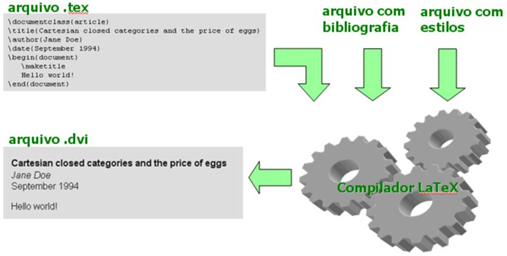
\includegraphics[scale=0.75]{Imagens/FiguraTeste.png}
% 	\textsf{\caption{Teste de uma figura em formato .png.}}
% 	\label{fig:FiguraTeste}
% \end{figure}

% \section{Operação interna e papel das expressões regulares}

% O funcionamento interno do módulo envolve a tradução de padrões \textit{RegEx}
% em operações de subgrafo sobre as estruturas moleculares representadas como
% grafos. Em termos gerais, o processo é dividido em etapas sucessivas que
% permitem converter descrições simbólicas de ligações e unidades
% monossacarídicas em estruturas compreensíveis computacionalmente.

% Primeiramente, ocorre a segmentação do padrão, na qual a expressão
% \textit{RegEx} fornecida é decomposta em módulos homogêneos, como unidades
% monossacarídicas ou ligações específicas. Por exemplo, o padrão
% \texttt{"Neu5Ac$\alpha$2-3Gal$\beta$1-4(Fuc$\alpha$1-3)GlcNAc"} é dividido em
% blocos como \texttt{"Neu5Ac$\alpha$2-3"}, \texttt{"Gal$\beta$1-4"} e
% \texttt{"Fuc$\alpha$1-3"}, representando diferentes segmentos estruturais que
% serão posteriormente analisados. Em seguida, ocorre a interpretação e expansão
% dos modificadores e quantificadores. Operadores como \texttt{+}, \texttt{*},
% \texttt{?}, intervalos \texttt{\{m,n\}} e quantificadores preguiçosos
% (\texttt{+?}) são suportados, permitindo definir repetições, ocorrências
% opcionais ou faixas de aparecimento dos motifs. Essa flexibilidade amplia a
% capacidade do módulo de reconhecer variações estruturais dentro de uma mesma
% família de glicanos. Posteriormente, aplica-se o processo de \textit{subgraph
% 	isomorphism}, em que cada segmento é buscado dentro do grafo que representa a
% estrutura glicosídica. Essa etapa utiliza algoritmos de isomorfismo de
% subgrafos para identificar correspondências exatas, mesmo em representações
% complexas que envolvem ramificações e múltiplas conexões entre unidades.

% Outro componente essencial é a implementação das operações de
% \textit{lookahead} e \textit{lookbehind}, herdadas das expressões regulares
% textuais. Elas permitem incluir ou excluir determinados contextos do padrão de
% busca sem incorporá-los ao resultado final, sendo cruciais para capturar motifs
% cuja ocorrência depende de um contexto estrutural específico.

% Por fim, ocorre a construção do caminho de correspondência, na qual um
% algoritmo iterativo reconstrói o trajeto contínuo dentro do grafo, unindo as
% correspondências parciais e validando os requisitos definidos pela expressão
% completa. Essa abordagem possibilita representar ligações específicas, como
% $\alpha$1-3 ou $\beta$1-6, bem como ambiguidade estrutural e ramificações
% expressas por meio de parênteses. Dessa forma, a notação \textit{RegEx} é
% adaptada à topologia molecular, permitindo uma modelagem altamente expressiva e
% precisa das estruturas glicosídicas.

\section{Vantagens da RegEx no contexto do \texttt{glycowork}}

Como comentado, a inovação trazida pelo \texttt{Glycan RegEx} ao framework
\texttt{glycowork} consiste na união do método tradicional de busca por motifs
com isomorfismo de subgrafo e o uso de um sistema de expressões regulares
específico para glicanos.

Sem o uso das expressões regulares, há a necessidade de uma base estática de
motifs já conhecidos - como pode ser vista no arquivo
\texttt{common\_names.json} do próprio framework -, o uso de muitas combinações
de padrões para detectar motifs complexos e específicos do glicano e a
dificuldade de capturar contextos maiores, como um motif presente apenas em um
ramo do glicano. Todos esses fatores culminam em um uso bastante rígido e, por
vezes, difícil de representar de forma computacional.

Com a introdução do sistema \texttt{Glycan RegEx} é possível escrever padrões
de buscas de motifs em um formato mais declarativo e eficaz, com uso de
operadores clássicos que permitem negação, repetição e demais operações. Dessa
forma, o algoritmo de busca de motifs tem a capacidade de gerar diversos
subgrafos intermediários (ao contrário do mecanismo anterior), encontrando a
combinação ideal de motifs de forma refinada e mais simples para o programador.

Esta camada adicional que o sistema traz pode gerar um \textit{overhead} em
estruturas mais simples do glicano quando comparado com a busca tradicional do
\texttt{glycowork} por motifs. Entretanto, quando aplicado em glicanos mais
complexos ou maiores, tal mecanismo se sobressai tanto em sua eficácia, podendo
ser mais simples escrever uma única expressão regular que atenda aos critérios,
quanto em sua eficiência.


	
	% Capitulo 3: Terceiro capítulo (arquivo Includes/Capitulo3.tex)
	% Capítulo 3
\chapter{Funções chave e eventos de código}

Para ilustrar o funcionamento do framework glycowork para expressões regulares 
de glicanos, exploraremos algumas de suas funções chave e apresentaremos 
exemplos de código.

\section{preprocess\_patern}

A função $preprocess\_pattern$ é responsável por transformar uma expressão 
regular de glicano em uma lista de "pedaços" ou componentes. Isso é crucial 
porque as expressões de glicanos podem conter modificadores, quantificadores e 
estruturas condicionais que precisam ser interpretadas corretamente antes da 
correspondência de padrões.

\begin{figure}[htb]
	\centering
  	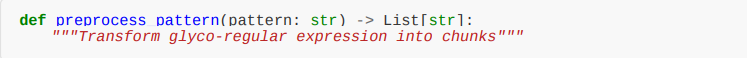
\includegraphics[scale=0.5]{Imagens/Figura 3_1.png}
  	\textsf{\caption{Implementação da função process\_pattern}}
  	\label{fig:implementação da função process\_pattern}
\end{figure}

\subsection{Exemplo de uso}

Considere a expressão regular de glicano $ex-HexNAc-([Hex|Fuc])\{1,2\}-HexNAc$. 
Esta expressão busca um padrão que começa com $Hex$, seguido por $HexNAc$, 
depois um ou dois $Hex$ ou $Fuc$, e termina com $HexNAc$.

\begin{figure}[H]
	\centering
  	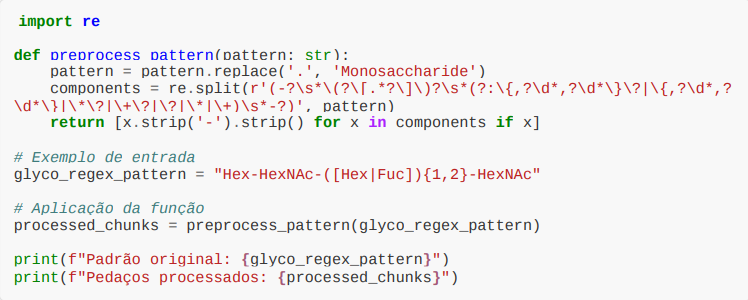
\includegraphics[scale=0.5]{Imagens/Figura 3_2.png}
  	\textsf{\caption{Aplicação da função process\_pattern}}
  	\label{fig:aplicação da função process\_pattern}
\end{figure}

\subsection{Comportamento de entrada}

Para a entrada $Hex-HexNAc-([Hex|Fuc])\{1,2\}-HexNAc$ , a função $preprocess\_pattern$ irá:
\begin{enumerate}
	\item Substituir qualquer $.$ por Monosaccharide;
	\item Dividir a string em componentes com base em um padrão de expressão 
		regular que identifica modificadores e quantificadores $( [Hex|Fuc] , {1,2} )$;
	\item Remover strings vazias e espaços em branco, além de hífens ( - ) das 
		extremidades dos componentes.
\end{enumerate}

O resultado esperado será uma lista de strings, onde cada string representa um 
"pedaço" da expressão regular de glicano, pronto para ser processado por outras 
funções do framework.

\section{specify\_linkages}

A função $specify\_linkages$ converte notações abreviadas de ligações em sua 
forma completa. Isso é essencial para padronizar as representações de glicanos 
e garantir que as operações de grafo possam interpretar corretamente as 
ligações entre os monossacarídeos.

\begin{figure}[htb]
	\centering
  	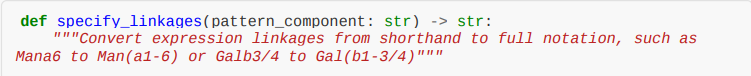
\includegraphics[scale=0.5]{Imagens/Figura 3_3.png}
  	\textsf{\caption{Implementação da função specify\_linkages}}
  	\label{fig:implementação da função specify\_linkages}
\end{figure}

\subsection{Exemplo de uso}

Considere um componente de padrão como $Mana6$ ou $Galb3/4$.

\begin{figure}[H]
	\centering
  	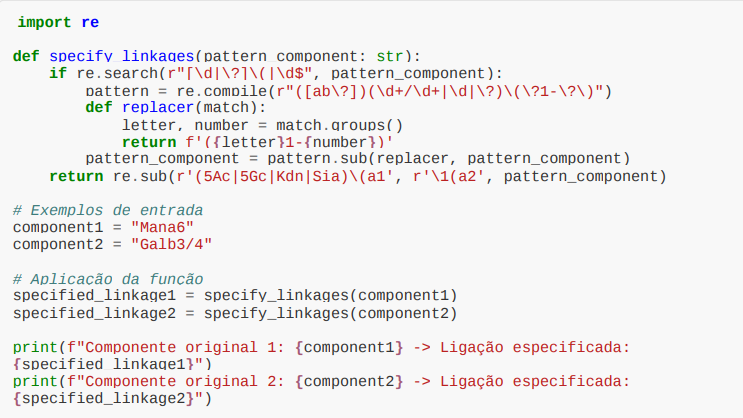
\includegraphics[scale=0.5]{Imagens/Figura 3_4.png}
  	\textsf{\caption{Aplicação da função specify\_linkages}}
  	\label{fig:aplicação da função specify\_linkages}
\end{figure}

\subsection{Comportamento de entrada}

Para $Mana6$, a função identificaria a notação abreviada e a converteria para 
$Man(a1-6)$. Similarmente, $Galb3/4$ seria convertida para $Gal(b1-3/4)$. Esta 
padronização é vital para a consistência na representação das ligações glicosídicas.

\section{get\_match}

A função $get_match$ é a principal interface para encontrar correspondências de 
uma expressão regular de glicano em uma estrutura de glicano. Ela utiliza as 
funções auxiliares como $preprocess_pattern$ e $specify\_linkages$ internamente 
para realizar a correspondência de padrões baseada em grafos.

\begin{figure}[htb]
	\centering
  	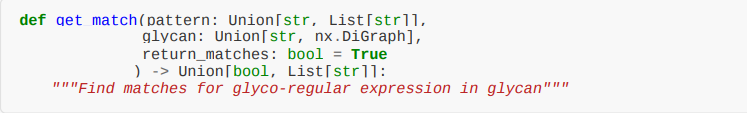
\includegraphics[scale=0.5]{Imagens/Figura 3_5.png}
  	\textsf{\caption{Implementação da função get\_match}}
  	\label{fig:implementação da função get\_match}
\end{figure}

\subsection{Exemplo de uso}

Para um exemplo prático de $get\_match$, precisaríamos de um ambiente glycowork 
completo, incluindo a capacidade de converter strings de glicanos em objetos 
networkx.DiGraph. No entanto, podemos ilustrar o conceito com um exemplo 
simplificado de como a função seria invocada e o tipo de resultado esperado.

\begin{figure}[H]
	\centering
  	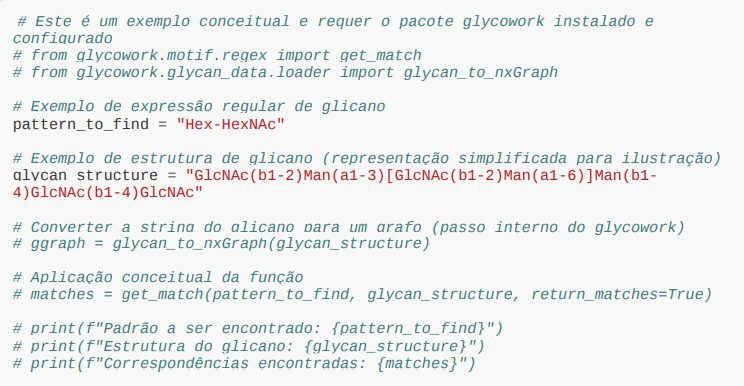
\includegraphics[scale=0.5]{Imagens/Figura 3_6.png}
  	\textsf{\caption{Aplicação da função specify\_linkages}}
  	\label{fig:aplicação da função specify\_linkages}
\end{figure}

\subsection{Comportamento de entrada}

Quando $get\_match$ é chamada com um pattern (expressão regular de glicano) e 
um glycan (estrutura de glicano), ela realiza os seguintes passos:

\begin{enumerate}
	\item Pré-processamento do Padrão: Utiliza $preprocess\_pattern$ para quebrar 
		a expressão regular em componentes;
	\item Conversão do Glicano: Se o glicano for fornecido como string, ele é 
		convertido para um objeto $networkx.DiGraph$, que é a representação interna 
		usada para operações de grafo;
	\item Correspondência de Padrões Baseada em Grafo: A função então executa um 
		algoritmo de correspondência de subgrafo para encontrar todas as ocorrências 
		do padrão dentro do grafo do glicano;
	\item Formatação dos Resultados: Se $return\_matches$ for True, a função 
		retorna uma lista de strings, onde cada string representa uma subestrutura 
		de glicano que corresponde ao padrão. Caso contrário, retorna um booleano 
		indicando se alguma correspondência foi encontrada.
\end{enumerate}

Este processo permite que o framework glycowork identifique padrões complexos em 
estruturas de glicanos, superando as limitações das expressões regulares textuais 
tradicionais ao considerar a topologia e as ligações químicas dos glicanos.
	
	% Capitulo 4: Quarto capítulo (arquivo Includes/Capitulo4.tex)
	% Capítulo 4
\chapter{Capítulo 4}

\section{Seção 1}

Teste para símbolo

\simb[$\lambda$ (algum símbolo)]{$\lambda$}


\section{Seção 2}

Teste para abreviatura 

\abrv[UFRN -- Universidade Federal do Rio Grande do Norte]{UFRN}

\abrv[DIMAp -- Departamento de Informática e Matemática Aplicada]{DIMAp}
	
	% Capitulo 5: Quinto capítulo (arquivo Includes/Capitulo5.tex)
	% Capítulo 5
\chapter{Capítulo 5}

\section{Seção 1}

Seção 1


\section{Seção 2}

Alguns exemplos de citação: 

Na tese de Doutorado de Paquete \cite{PaquetePhD}, discute-se sobre algoritmos de busca local estocásticos aplicados a problemas de Otimização Combinatória considerando múltiplos objetivos. Por sua vez, o trabalho de \cite{KnowlesBoundedLebesgue}, publicado nos anais do IEEE CEC de 2003, mostra uma técnica de arquivamento também empregada no desenvolvimento de algoritmos evolucionários multi-objetivo, trabalho esse posteriormente estendido para um capítulo de livro dos mesmos autores \cite{KnowlesBoundedPareto}. Por fim, no relatório técnico de \citeonline{Jaszkiewicz}, fala-se sobre um algoritmo genético híbrido para problemas multi-critério, enquanto no artigo de jornal de Lopez \textit{et al.} \cite{LopezPaqueteStu} trata-se do \textit{trade-off} entre algoritmos genéticos e metodologias de busca local, também aplicados no contexto multi-critério e relacionado de alguma forma ao trabalho de Jaszkiewicz (\citeyear{Jaszkiewicz}).

Outros exemplos relacionados encontram-se em \cite{Silberschatz} (livro), \cite{DB2XML} (referência da Web) e \cite{Angelo} (dissertação de Mestrado).

\subsection{Subseção 5.1}

Subseção 5.1


\subsection{Subseção 5.2}

Subsection 5.2


\section{Seção 3}

Seção 3
		
	% Consideracoes finais
	% Considerações finais
\chapter{Considerações finais}

As considerações finais formam a parte final (fechamento) do texto, sendo dito de forma resumida (1) o que foi desenvolvido no presente trabalho e quais os resultados do mesmo, (2) o que se pôde concluir após o desenvolvimento bem como as principais contribuições do trabalho, e (3) perspectivas para o desenvolvimento de trabalhos futuros, como listado nos exemplos de seção abaixo. O texto referente às considerações finais do autor deve salientar a extensão e os resultados da contribuição do trabalho e os argumentos utilizados estar baseados em dados comprovados e fundamentados nos resultados e na discussão do texto, contendo deduções lógicas correspondentes aos objetivos do trabalho, propostos inicialmente.


\section{Principais contribuições}

Texto.


\section{Limitações}

Texto.


\section{Trabalhos futuros}

Texto.
	
	% Bibliografia (arquivo Capitulos/Referencias.bib)
	\bibliography{Capitulos/Referencias}
	\bibliographystyle{abnt-alf}
	
	% Apêndice A (arquivo Includes/ApendiceA)
	% Apêndice
\apendice
\chapter{Primeiro apêndice}

Os apêndices são textos ou documentos elaborados pelo autor, a fim de complementar sua argumentação, sem prejuízo da unidade nuclear do trabalho.
	
	% Anexo A (arquivo Includes/AnexoA)
	% Anexo
\anexo
\chapter{Primeiro anexo}

Os anexos são textos ou documentos não elaborado pelo autor, que servem de fundamentação, comprovação e ilustração.
	
	% Página em branco
	\newpage

\end{document}